% https://towardsdatascience.com/a-comprehensive-guide-to-convolutional-neural-networks-the-eli5-way-3bd2b1164a53
% https://github.com/OValery16/Tutorial-about-3D-convolutional-network
\documentclass{report}

\usepackage{enumitem}  % package for description with bullets
\usepackage{graphicx}  % package for importing images
\usepackage{mathtools} % package for math equation
\usepackage{mathrsfs}  % package for math font
% \usepackage{amsmath}

\graphicspath{ {./} }
\begin{document}

\chapter {Convolutional Neural Networks}
As metioned before, Artificial Intelligence has been witnessing a monumental growth in bridging the gap between the capabilities of humans
and machines. Researchers and enthusiasts alike, work on numerous aspects of the field to make amazing things happen. One of many such areas
is the domain of Computer Vision. \\
The agenda for this field is to enable machines to view the world as humans do, perceive it in a similar manner and even use the
knowledge for a multitude of tasks such as Image/Video Recognition, Image Analysis and Classification, Media Recreation etc. The
advantages in Computer Vision with Deep Learning has been constructed and perfected with time primarily over one particular algorithm,
\textbf{a Convolutional Neural Network}.

\section {2D Convolutional Neural Network}
A Convolutional Neural Network (ConvNet/CNN) is a Deep Learning algorithm which can take in an input image, assing importance (learning
weights and biases) to various aspects/objects in the image and be able to differentiate one from the other. The pre-processing required
in a ConvNet is much lower as compared to the other classification algorithms. While in primitive method filters are hand-engineered,
with enough training, ConvNets have the ability to learn these filters/characteristics.

The architecture of a ConvNet is analogous to that of the connectivity pattern of Neurons in the Human Brain and was inspired by the
structure of the Visual Cortex. However, most ConvNets costist mainly in 2 parts:
\begin{description}[font=$\bullet$\scshape\bfseries]
\item [ Feature extractor] : \\
  This part of the network takes as input the image and extract features that are meaningful for its classification. It amplifies aspects
  of the input that are important for discrimination and suppresses irrelevant variations. Usually, the feature extractor cosists of
  several layers. For instance, an image which could be seen as an array of pixel values. The first layer often learns reprensations
  that represent the presence or absence of edges at particular orientations and locations in the image. The second layer typically
  detects motifs by spotting particular arrangements of edges, regardeless of small variations in the edge positions. Finally, the third
  may assemble motifs into larger combinations that correspond to paths of familiar objects, and subsequent layers would detect objects
  as combinations of these parts.
  
\item [ Classifier ] : \\
  This part of the network takes as input the previously computed features and use them to predict the correct label.
\end{description}

\begin{figure}[h]
  % 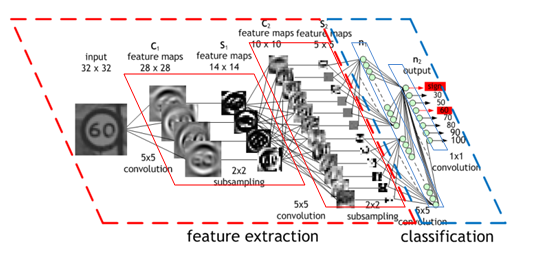
\includegraphics[scale=0.7]{convolutional_neural_network_structure} \]
  \centering
  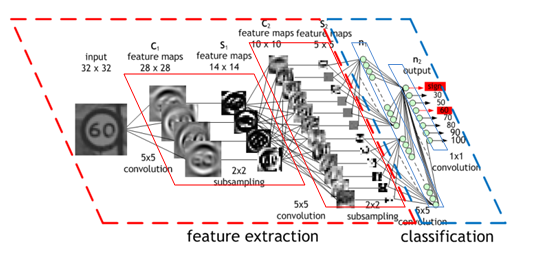
\includegraphics[scale=0.7]{convolutional_neural_network_structure}
  \caption{Typical structure of a ConvNet}
\end{figure}

In order to extract such features, ConvNets use 2D convolution operations.

\paragraph{Convolution}
\begin{figure}[h]
  \centering
  \begin{minipage}[b]{0.4\textwidth}
    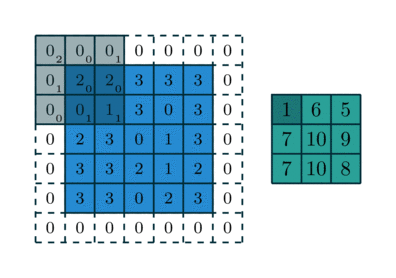
\includegraphics[width=\textwidth]{conv_1}
  \end{minipage}
  \hfill
  \begin{minipage}[b]{0.4\textwidth}
    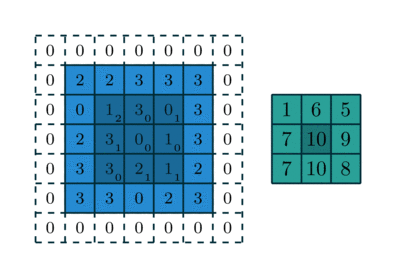
\includegraphics[width=\textwidth]{conv_2}
  \end{minipage}
  \caption{Convolution with kernel size:3, stride:2, padding:1}

\end{figure}


\section {3D Convolutional Neural Network}
Traditionally, ConvNets are targeting RGB images (3 channels). The goal of 3D CNN is to take as input a video and extract features from it.
When ConvNets extract the graphical characteristics of a single image and put them in a vector (a low-level representation), 3D ConvNets
extract the graphical characteristics of a set of images. 3D CNNs takes in to account a temporal dimension (the order of the images in the
video). From a set of images, 3D CNNs find a low-level representation of a set of images, and this representation is useful to find the
right label of the video (a given action is performed). \\
In order to extract such features, 3D ConvNets  use 3D convolution operations.

\begin{figure}[h]
  % 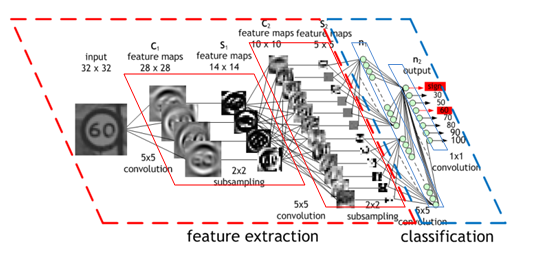
\includegraphics[scale=0.7]{convolutional_neural_network_structure} \]
  \centering
  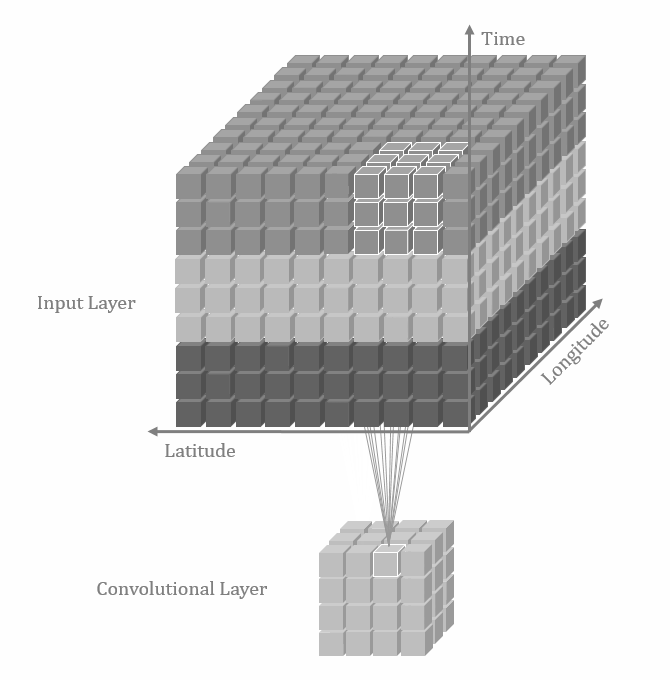
\includegraphics[scale=0.3]{3d_conv}
  \caption{3D Convolution operation}
\end{figure}

There are several existing approaches to tackle the video classification. This is a nonexaustive list of existing approaches:
\begin{description} [font=$\bullet$\scshape\bfseries]
\item[ ConvNets + LSTM cell] : Extract features from each frame with a ConvNet, passing the sequence to an RNN
\item[ Temporal Relation Networks] : Extract features from each frame with a ConvNet and pass the sequence to an MLP
\item[ Two-Stream Convolutional Networks] : Use 2 CNN, 1 spatial stream ConvNet which process one single frame at a time, and 1 Temporal stream ConvNet which process multi-frame optical flow
\end{description}
\end{document}
